\subsection{Hyperparameter Optimization}
There are five hyperparameters which influence the execution of \textit{SPIND}. The size of the initially created chunks (\textit{CHUNK}), the maximal number of values which are kept in main memory during the sorting phase per thread (\textit{SORT}), the maximal number of files which are merged at once per thread (\textit{MERGE}), the queue size for each relation during candidate validation (\textit{VALIDATION}) and the degree of parallelization (\textit{PARALLEL}). Leveraging Bayesian optimization \cite{shahriari2015taking}, we seek to efficiently and iteratively identify parameter configurations that minimize the execution time of \textit{SPIND} of various datasets. We lower bound \textit{CHUNK} by 10,000 to avoid the creation of a massive amount of files and set an upper bound of 100 million. We limit \textit{SORT} between 10,000 and 3.5 million to find a balance between a large number of files being written and a safe number under the main memory threshold. \textit{MERGE} is lower bounded by two and upper bounded by 1,000 to not put too much pressure on the file system. \textit{VALIDATION} is upper bounded by 1 million. Finlay, \textit{PARALLEL} is upper bounded by the number of virtual threads of the executing machine.

A first observation is that \textit{PARALLEL} has a clear negative correlation with the execution time. Regardless of how the other four parameters are set. Figure \ref{fig:parallelization_effectivness} shows a group of hex-bin plots, where the y-Axis is always the degree of parallelization and the x-Axis take on the other variables. After X?X iterations, our estimated multi-variable function has a maximal $2\sigma$ uncertainty of X?X. These observations lead to the decision of fixing \textit{PARALLEL} to its upper bound.

The next iteration yields that \textit{CHUNK} is the second most important variable. While smaller chunks strictly correlate with the total number of files being created and therefore also the I/O overhead, we find an optimum at a chunk size of five million which is robust over different datasets. A smaller chunk size enables more tasks to be processed in parallel which has been shown to overcome the I/O operations at some point.

Summarizing the last three iterations, we find that \textit{SORT} and \textit{VALIDATION} should be as large as possible under the given main memory constraints. The results for \textit{MERGE} X?X %TODO

In Figure \ref{fig:chunk_size} we can observe the relative change in the number of files created under changing chunk sizes (left) and the relative execution times compared to the longest run (right). For these experiments, we always average the execution of three runs.

\begin{figure}
    \centering
    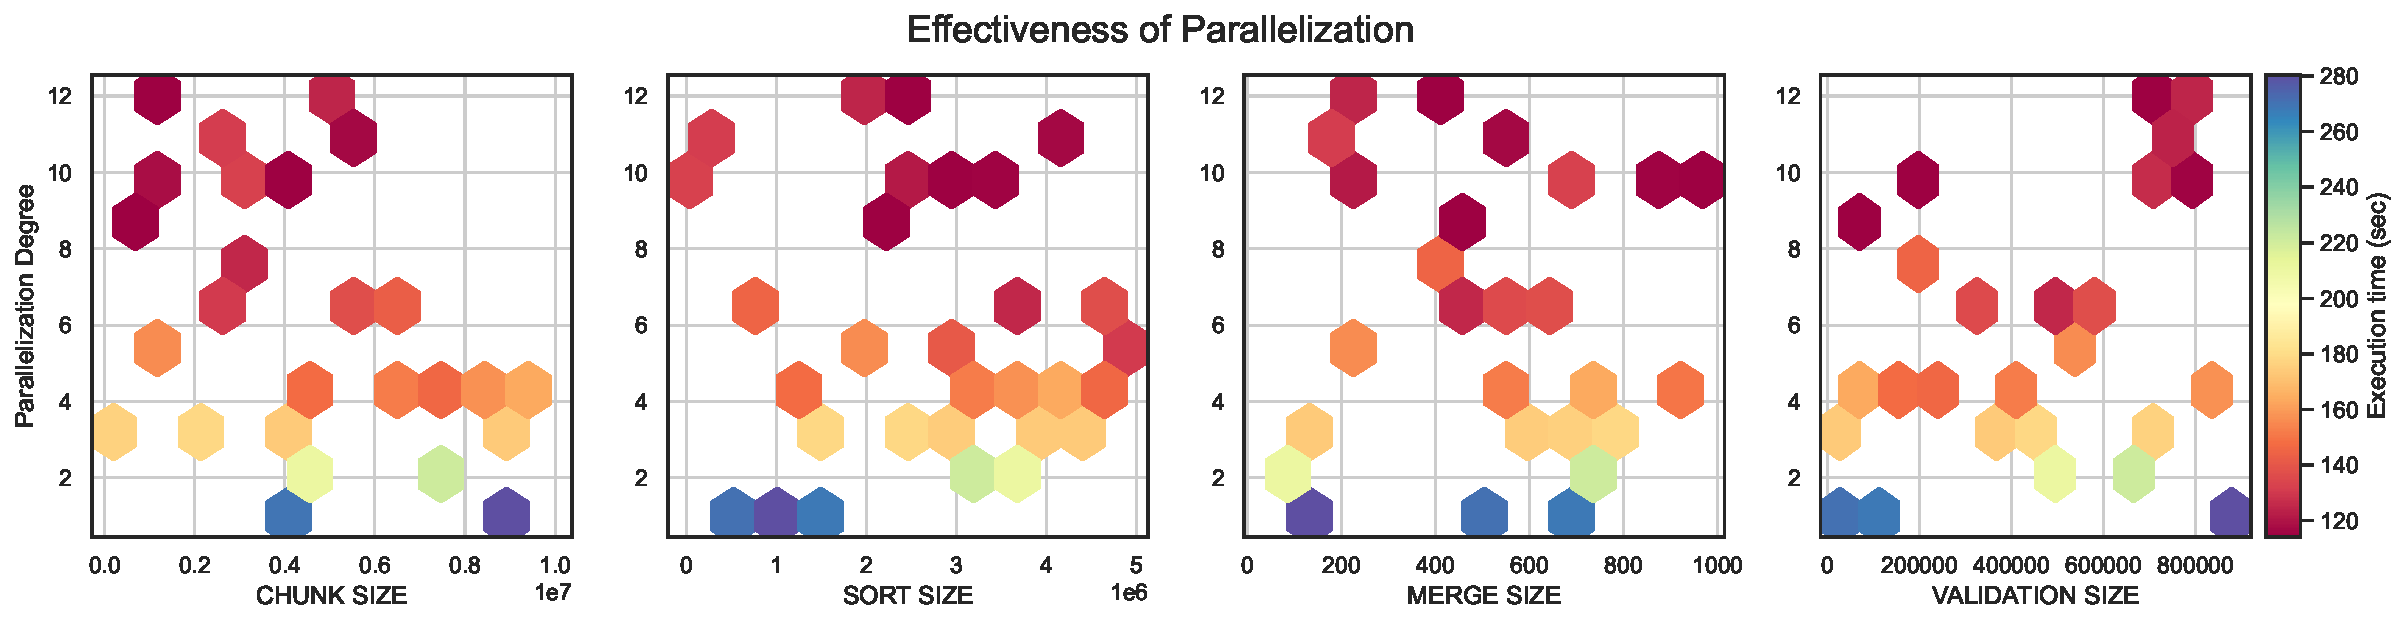
\includegraphics[width=.47\textwidth]{figures/parallelization.pdf}
    \caption{Effectiveness of the parallelization degree regardless of any other parameter.}
    \label{fig:parallelization_effectivness}
\end{figure}

\begin{figure}
    \centering
    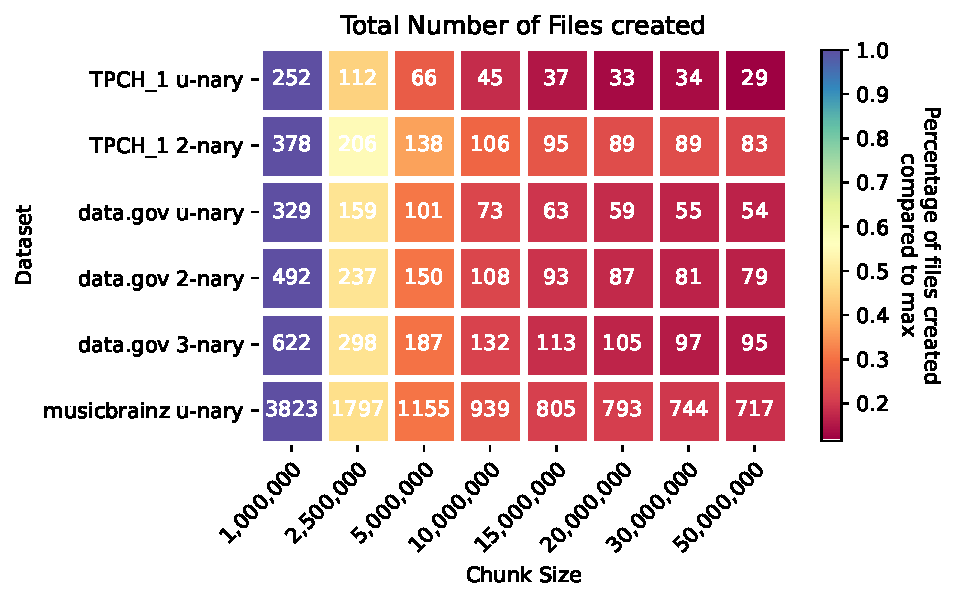
\includegraphics[width=.47\textwidth]{figures/chunk_size_files_created.pdf}
    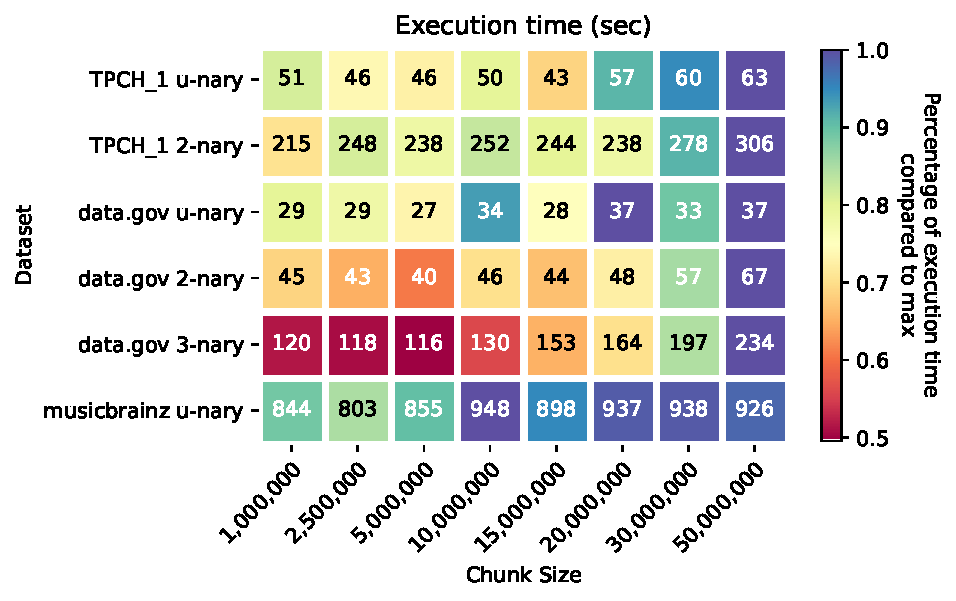
\includegraphics[width=.47\textwidth]{figures/chunk_size_execution_time.pdf}
    \caption{Files created (top) and execution time (bottom) under varying chunk sizes. Both relative to the maximum.}
    \label{fig:chunk_size}
\end{figure}